% !TEX program = xelatex
\documentclass[a4paper, 10]{article}
% include some packages
\usepackage{graphicx, color, pgfplots, pgf-umlsd, ifthen}
\usepackage{float}
\usepackage[]{fp}
\usepackage{amsmath, amsfonts, amssymb}
\usepackage{tikz}
\usepackage[UTF8]{ctex}
\usepackage{hyperref}
\usepackage{xcolor}

% Change settings for caption
\renewcommand{\figurename}{Figure}
\renewcommand{\tablename}{Table}

% Path for my images
\graphicspath{{./images/}}

% infos about the doc
\begin{document}
\title{HW3: CNN Implementation}
\author{王昊文}

\maketitle


% Document starts here
\section{Overview}
    In this homework, I will be implementing a simple CNN from scartch by 
    using only Numpy, the model will be evaluated on a simple 3-class fruit 
    image dataset. \\
    \indent The whole homework strictly follows the object-orientated philosophy, which 
    treats \emph{datatset}, \emph{data loader}, \emph{trainer}, \emph{logger} as 
    different objects, so that it can be very convinient to write your own custom
    objects. You can combine all your settings and put them under \verb|config.json|
    inside the root folder. \\ 
    \indent Also, you will find that the structure is highly similar to 
    \href{https://github.com/victoresque/pytorch-template}{pytorch template},
    which allows me to have a basic building block to build this project.
    
\section{Details}
    \subsection{Data}
        In the fruit dataset, we have a total of 1471 of training data,
        and 498 testing data. Each image in the dataset has a height and 
        width of 32, and each image contains four channels, the first
        three represents RGB, and the last channel is the alpha value, 
        which represents the transparency of each color. However, the 
        alpha value will not be used in the CNN, so will be dropped
        will doing preprocessing. \\
        \indent There are 3 types of the fruits, they are: Carambola, 
        Lychee, Pear.

    \subsection{Model}
        \subsubsection{Intuition and loss function selection} 
            This is a simple task, since there are only three classes, so I will be 
            implementing a light, shallow CNN network for this task. The model acheives
            great results as we will discuss it later in the report, despite its shallowness.
            \indent For the loss function, it is obvious that Softmax with cross-entropy
            loss is the best choice for this task.
        \subsubsection{Architecture} 
            Note that is defined under \verb|model.py|. The total trainable parameters is
            1,050,227. More details are listed in table \ref{table:1}. 
            \begin{table}[h!]
                \centering
                \begin{tabular}{|c|c|c|}
                    \hline
                    Layer               &   Output Shape               & Param Num. \\
                    \hline
                    Conv2d-1            &   [16, 8, 32, 32]            & 224 \\
                    ReLU-2              &   [16, 8, 32, 32]            & 0 \\
                    Conv2d-3            &   [16, 16, 32, 32]           & 1,168 \\
                    ReLU-4              &   [16, 16, 32, 32]           &     0 \\
                    Linear-5            &   [16, 64]                   & 1,048,640 \\
                    ReLU-6              &   [16, 64]                   &     0 \\
                    Linear-7            &   [16, 3]                    & 195    \\
                    \hline
                \end{tabular}
                \caption{A list of the layers of the current model}
                \label{table:1}
            \end{table}
            Note that all convolution have a kernel size of 3, stride 1 and 0 padding.

    \subsection{Training and validation}
            As shown in figure \ref{fig:2}, our loss curve converged
            really quickly in just a few epochs. As for the accuracy
            shown in figure \ref{fig:3}, The model started out at around
            $60\%$ and quickly reached $100\%$ near 10 epochs. When training, 
            I set the batch size to 32. During training, I used SGD as the 
            optimizer, with learning rate of $10^{-3}$. Also, the learning 
            rate is scheduled to decay at a rate of $10^{-6}$. \\
            The above training details shows great results.
    \begin{figure}[H]
        \centering
        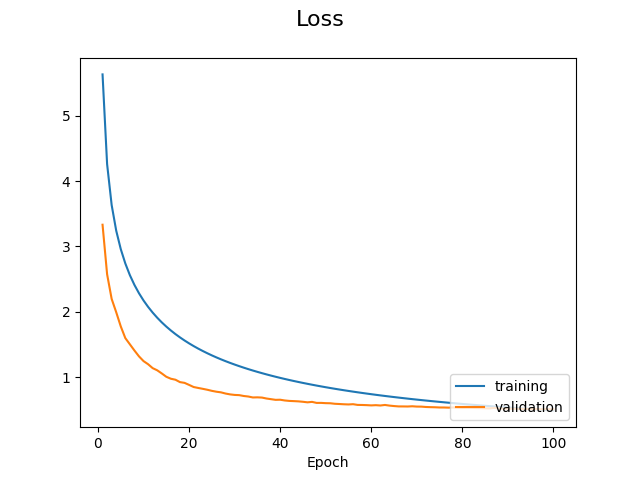
\includegraphics[scale=0.7]{Loss.png}
        \caption{The cross-entropy loss curve of the model} \label{fig:2}
    \end{figure}
    \begin{figure}[H]
        \centering
        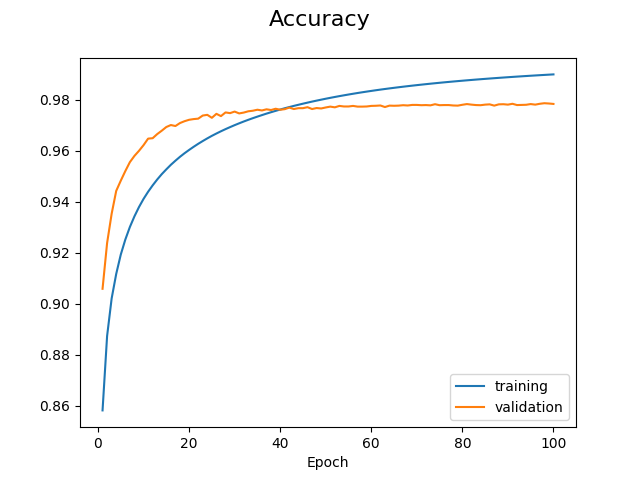
\includegraphics[scale=0.7]{Accuracy.png}
        \caption{The accuracy curve of our model} \label{fig:3}
    \end{figure}
    \subsection{Performace}
        I have provided a best model \verb|checkpoint-epoch40.pth| and the config 
        \verb|config.json| under the root folder. You can view  the testing accuracy 
        by using the \verb|test.py| given under the root folder. You can also 
        use \verb|checkpoint-epoch5.pth|, this is a mid-product while 
        training, which has only $89\%$ accuracy to show that the accuracy 
        results are correct.
        \begin{figure}[H]
            \centering
            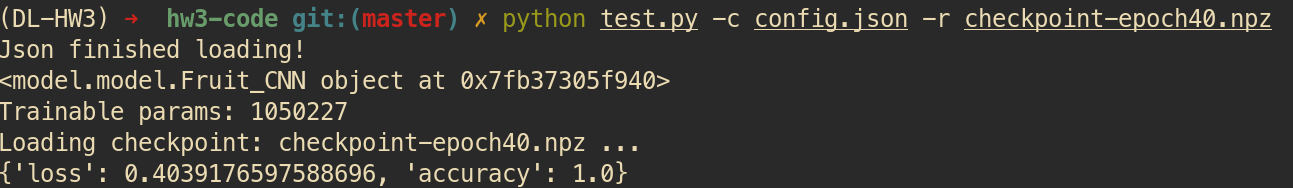
\includegraphics [scale=0.3]{Screenshot_20220111_143520.png}
            \caption{Results on our testing set}
        \end{figure}
\section{Result Visualization}
    In this part, we will show something other than the loss and accuracy.
    We will show the feature map of the 2 convolutions to visualize
    what the network is doing.\\
    \indent In the first row, it consists the input image and the 
    three channels it has. The second and the third row are
    4 of the 8 channels from our CNN layers. We can see that
    the first Convolution is extracting the overall feel from
    the input image, and the second Convolution can sort of getting
    the shape of the image.
    \begin{figure}[H]
        \centering
        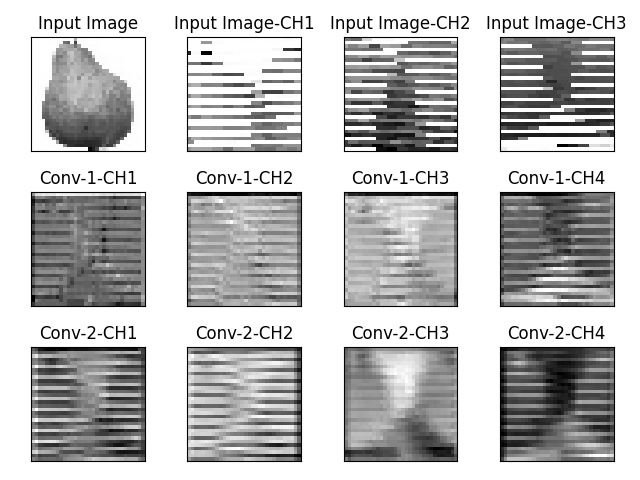
\includegraphics[width=\textwidth]{Pear.png}
        \caption{Pear 1} \label{fig:4}
    \end{figure}
    \begin{figure}[H]
        \centering
        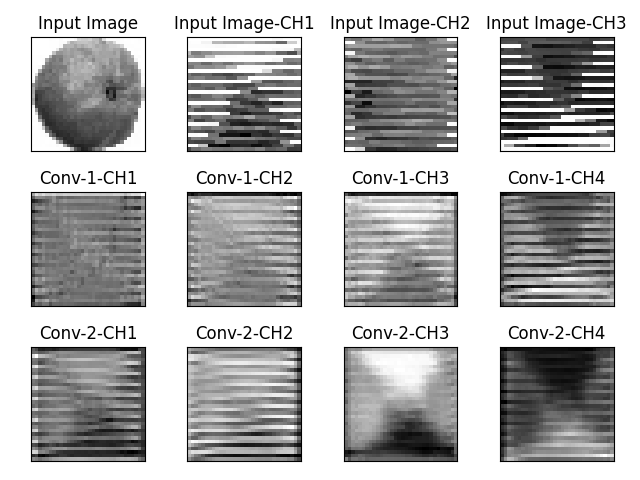
\includegraphics[width=\textwidth]{Pear1.png}
        \caption{Pear 2} \label{fig:5}
    \end{figure}
    \begin{figure}[H]
        \centering
        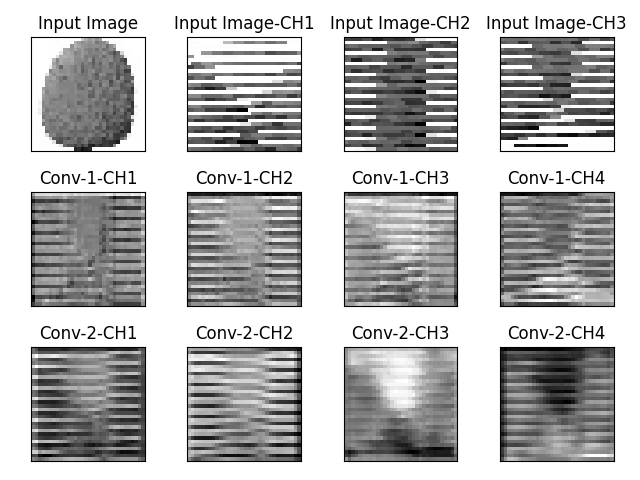
\includegraphics[width=\textwidth]{Lychee.png}
        \caption{Lychee 1} \label{fig:6}
    \end{figure}
    \begin{figure}[H]
        \centering
        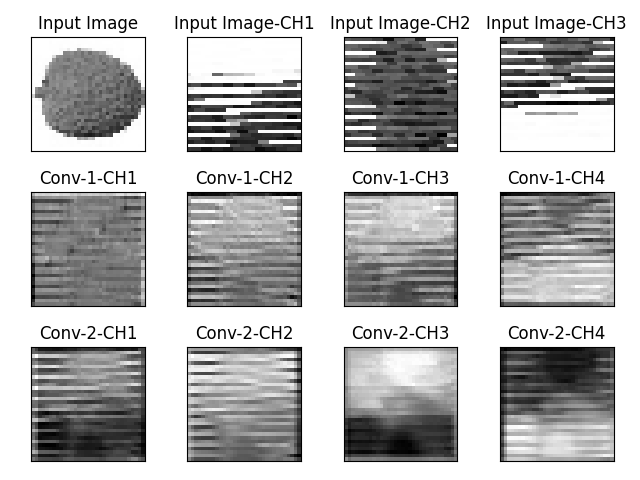
\includegraphics[width=\textwidth]{Lychee1.png}
        \caption{Lychee 2} \label{fig:7}
    \end{figure}
    \begin{figure}[h]
        \centering
        \includegraphics[width=\textwidth]{carambola.png}
        \caption{Carambola 1} \label{fig:8}
    \end{figure}
    \begin{figure}[h]
        \centering
        \includegraphics[width=\textwidth]{carambola1.png}
        \caption{Carambola 2} \label{fig:9}
    \end{figure}
\section{Challenges}
    In the process of writing this homework, The hardest part
    is definitely implementing the convolution operation.
    At first, I wrote a triple for loop implementation(width, heght,
    number of kernels). However, that took forever to train with 
    only CPU. So after closer incpection on the vectorized numpy
    code and some really tricky techniques, to stack up all the 
    input and layers, I was able to nearly 10 times the speed
    on doing convolution. \\
    \indent The most interesting part is looking at the feature maps.
    This really gives insight of what our Convolution layers are
    looking at. However it took me quite a while to correctly 
    show the feature maps, with only the matplotlib library.
\end{document}
